\chapter{Introduction}
\label{chap:Introduction}
Software bugs are an inherent part of programming, often leading to unexpected behaviour and system failures. Debugging these errors is a \textit{time-consuming} process taking between 20-60\% of active work time \cite{DebugTimeSelfReport}, with programmers spending a \textit{highly skewed} proportion of their time identifying and resolving a small proportion of \textit{difficult} bugs \cite{DebugSkew}.

Type systems aim to alleviate some of this burden by classifying expressions and operations that are allowed to work on them. This may be done \textit{statically} at compile time or \textit{dynamically} during runtime. The expressions not conforming to the type system manifest themselves as \textit{type errors}.

In static typing, blame for type errors are typically localised to a single location in the code. However, this localisation may be misleading, as the actual cause of the error might be rooted in a broader context, for example in OCaml 65\% of type errors related to \textit{multiple} locations \cite{StudentTypeErrorFixes}. Additionally, the errors only \textit{state} the expected types, but with no explanation for \textit{why}.

In dynamic typing, type errors are found later only appearing during runtime with specific inputs.
Additionally, they don't generally specify any source code context which caused them. However, such an error is accompanied by an evaluation trace, which can be \textit{more intuitive} \cite{TraceVisualisation}, demonstrating concretely why values are ill-typed programs go wrong.

\paragraph{Aims} This project seeks to improve user understanding of type errors by explaining static type errors more \textit{completely}, and \textit{combining} the benefits of static and dynamic type errors. I consider three directions to achieve this, implementing three features to achieve them for use in the Hazel language \cite{Hazel}:
\begin{enumerate}
\item Can we explain \textit{static type errors} more \textit{completely}, highlighting the code that determines \textit{why} the error expects it's inconsistent type? 

Being more \textit{complete}, this would alleviate the issue of static errors being incorrectly localised, while also helping build understanding of \textit{why} the errors occur.

\textbf{Solution:} I devise a \textit{novel} method: \textbf{type slicing}. Including formal mathematical foundations built upon the formal \textit{Hazel calculus} \cite{HazelLivePaper}. Additionally, it generalises to highlight all code relevant to typing any expressions (not just errors).

\item Can we track source code which contributes to a \textit{dynamic type error}?

This would provide missing source code context to understand how types involved in a dynamic type error originate from the source code.

\textbf{Solution:} I devise a \textit{novel} method: \textbf{cast slicing}. Also having formal mathematical foundations. Additionally, it generalises to highlight source code relevant to requiring any specific runtime casts.

\item Can we provide dynamic evaluation traces to explain \textit{static type errors}?

This would provide an \textit{intuitive} concrete explanation for static type errors.

\textbf{Solution:} I implement a \textbf{type error witness search procedure}, which discovers inputs (witnesses) to expressions which cause a \textit{dynamic type error}. This is based on research by Seidel et al. \cite{SearchProc} who devised and evidenced the usefulness of a similar procedure for a subset of OCaml.
\end{enumerate}

Hazel \cite{Hazel} is a functional, locally inferred, and gradually typed research language that allows writing \textit{incomplete programs} under active development at the University of Michigan. Being gradually typed, it is a natural choice for this project, allowing both static and dynamic code to coexist. I successfully demonstrate the utility of these three features in improving understanding of \textit{both} static and dynamic errors as well as how the two classes of errors interact and may be linked automatically.

%\paragraph{Example} \Cref{fig:ErrorExample} shows an attempt at writing an int list concatenation function. But list cons (\code{::}) is used instead of list concatenation (\code{@}). Type slicing will automatically highlight the code that caused \code{x} to synthesise the \code{[Int]} type and the code that enforces the requirement that \code{x} is an \code{Int}. If the error is still not clear, the search procedure can be used to generate inputs which evaluate to cast errors, for example \code{concat([[], []])}, giving a concrete evaluation trace to an error. Finally, cast slicing will allow the cast errors to be selected, highlighting source code that enforced the cast, potentially giving a more concise slice than statically computed by type slicing. The results of this example among others are explored in the evaluation (\cref{sec:EvalExamples}).

%\begin{figure}[h]
%\centering
%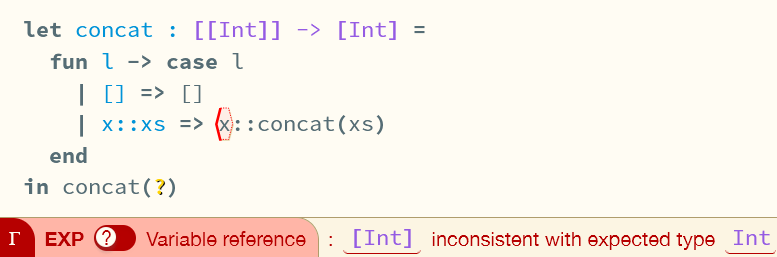
\includegraphics[width=0.7\textwidth]{Media/Figures/concat_error}
%\caption{A Static Type Error from the Hazel Editor}
%\label{fig:ErrorExample}
%\end{figure}

\begin{figure}
\centering
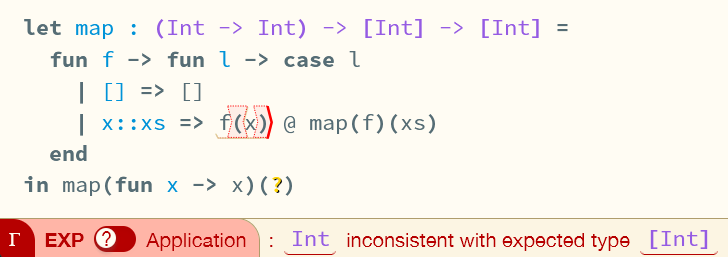
\includegraphics[width=0.75\textwidth]{Media/Figures/map_example_intro}

Note: \code{?} represents a hole, an \textit{incomplete} part of the program.
\caption{\textbf{Example:} Concatenation \code{@} has been used instead of cons \code{::}, but \code{f(x)} is incorrectly localised as the error. Type slicing will give a full context highlighting the terms involved in the error (the annotation, \code{f(x)} and \code{@} operator). The search procedure could find a witness (e.g. \code{[0]}) concretely evaluating to a dynamic error. The cast in the dynamic error will contain a slice highlighting the source code that makes \code{@} take lists as input. The results are demonstrated in the evaluation \cref{sec:EvalExamples}}.
\end{figure}

\section{Related Work}
\label{sec:RelatedWork}
There has been extensive research into the field of programming languages and debugging, attempting to understand \textit{what} is needed \cite{DebugNeeds}, \textit{how} developers fix bugs \cite{HowFixBugs}, and a plethora of compiler improvements and tools. This project builds adds to this body of research in new ways, focusing on the Hazel language which is itself an active research project being taken in various directions but of particular note as a \textit{teaching language} \cite{HazelTutor} for students; these features can additionally help with building understanding of bidirectional type systems. 

To my knowledge the ideas of \textit{type slicing} and \textit{cast slicing} are novel. However, they were inspired, but differing substantially, to \textit{program slices}, originally explored by Weiser \cite{ProgSlice}, slices in expression-based languages \cite{FunctionalProgExplain}, \textit{dynamic program slicing} \cite{DynProgSlice} and \textit{type error slicing}\cite{ErrSlice, HaackErrSlice}, which similarly relate to type systems.

The \textit{type witness search procedure} is	 based upon Seidel et al. \cite{SearchProc}, but with significant differences, which will be explained throughout.